\documentclass[a4paper,11pt,exos]{nsi} % COMPILE WITH DRAFT
\usepackage{pifont}
\usepackage{fontawesome5}
\usepackage{hyperref}



\begin{document}
\classe{\terminale Comp}
\titre{Exercices - Intégration}
\maketitle

\tabularstyled[UGLiBlue]
\begin{tabular}{p{16.5cm}}
    \rowcolor{UGLiBlue}
    \ths Capacités attendues : \\

    \ding{111} Estimer graphiquement ou encadrer une intégrale, une valeur moyenne.   \\
    \ding{111} Calculer une intégrale, une valeur moyenne \\
    \ding{111} Calculer l’aire sous une courbe ou entre deux courbes.\\
    \ding{111} Interpréter une intégrale, une valeur moyenne dans un contexte issu d’une autre discipline.\\
\end{tabular}


\vspace*{.5cm}

\subsection*{Intégrale comme aire sous une courbe}

\dleft{10cm}{
    \exo{}
    Sur le graphique ci-contre sont données la droite représentant une fonction $f$ ainsi qu'une surface colorée.\\
    Déterminer par lecture graphique la valeur de l'intégrale $\displaystyle \int_{-3}^1 f(x) \, dx$.
}
{
    \def\xmin{-4} \def\ymin{-1}\def\xmax{2}\def\ymax{3}
    \def\F{2}
    \begin{tikzpicture}
    \draw[fill=white] (\xmin,\ymin) rectangle (\xmax,\ymax);
        \draw[fill = UGLiOrange!30](-3,0) rectangle (1,2);
        \repereal{\xmin}{\ymin}{\xmax}{\ymax}
        \clip (\xmin,\ymin) rectangle (\xmax,\ymax);
        \draw[UGLiRed,domain=-3:1,smooth,variable=\x,thick] plot ({\x},{\F});
    \end{tikzpicture}
}

\dleft{10cm}{
    \exo{}
    Calculer la valeur de l'intégrale $\displaystyle \int_{0}^4 (-x+4) \, dx$.
}
{
    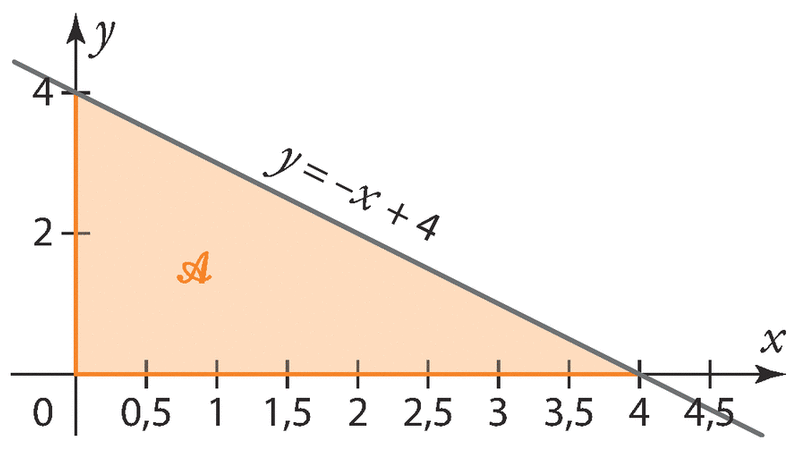
\includegraphics[width=6cm]{Sesamath30p152.png}
}

\exo{}

\exo{}
	
		\begin{minipage}{6.5cm}
			\def\xmin{-2}	\def\xmax{4}	\def\ymin{-1}	\def\ymax{5}
			\def\F{-(\x+1)*(\x-3)}
			\begin{tikzpicture}
				\repereal{\xmin}{\ymin}{\xmax}{\ymax}
				\clip	(\xmin,\ymin) rectangle (\xmax,\ymax);
				\fill[pattern =north east lines, pattern color = blue] 	(-1,0) --
				plot[thick,domain=-1:2,smooth,variable=\x] ({\x},{\F}) --
				(2,3)-- (2,0) --cycle;
				\draw[thick,domain=\xmin:\xmax,smooth,variable=\x]  plot ({\x},{\F});
			\end{tikzpicture}
		\end{minipage}
		\begin{minipage}{10.5cm}
			Voici la courbe représentative d'une fonction $f$ dans un repère orthonormal $\repaff$.\\
			On note $$\displaystyle I=\int_{-1}^{2}f(x)\text{d}x$$
			\begin{enumerate}
				\item 	Encadrer $I$ par 2 entiers.
				\item 	Quelle est l'amplitude de cet encadrement ?
			\end{enumerate}
		\end{minipage}
	
	\exo{}
	
\begin{minipage}{6.5cm}
	\def\xmin{-2}\def\xmax{4}\def\ymin{-1}\def\ymax{6}
	\def\F{5+(\x+1)*(\x-3)}
	\begin{tikzpicture}
	\reperea{\xmin}{\ymin}{\xmax}{\ymax}
	\clip	(\xmin,\ymin) rectangle (\xmax,\ymax);
	\fill[pattern =north east lines, pattern color = blue] 	(0,0)-- (0,2) --
	plot[thick,domain=-0:3,smooth,variable=\x] ({\x},{\F}) --(3,5)-- (3,0) --cycle;
	\draw[thick,domain=\xmin:\xmax,smooth,variable=\x]  plot ({\x},{\F});
	\end{tikzpicture}
\end{minipage}
\begin{minipage}{10.5cm}
	Voici la courbe représentative d'une fonction $g$ dans un repère orthonormal $\repaff$.\\
On note $$\displaystyle J=\int_{0}^{3}g(x)\text{d}x$$
\begin{enumerate}
	\item 	Encadrer $J$ par 2 entiers.
	\item 	Quelle est l'amplitude de cet encadrement ?
	\item 	Encadrer $J$ par 2 multiples de $0,25$ (compter les petits carreaux).
	\item 	Quelle est l'amplitude de cet encadrement ?
\end{enumerate}
\end{minipage}	

\end{document}